\section{Surajustement}
\subsection{Le phénomène}
Lorsque un réseau de neurones à apprentissage supervisé apprend de trop nombreuses fois à partir du même set d'exemple, alors il se produit un phénomène appelé \emph{surajustement}.\cite{statistica}
Le réseau devient dès lors de moins en moins efficace sur des entrées non rencontrées pendant les phases d'apprentissage.
La Figure \ref{interruption} montre qu'au fil des cycles d'apprentissages, l'erreur diminue.
À un certain moment, l'erreur sur des paires entrée/sortie non fournies pendant la phase d'apprentissage augmente. 
C'est à partir de là que le réseau de neurones surajuste.
\begin{figure}
 \centering
 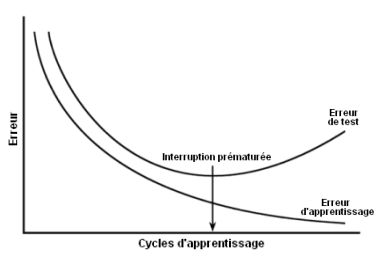
\includegraphics[scale=0.6]{../figures/surgeneralisation.jpg}
 \caption{Interruption prématurée. \textbf{Source}: STATISTICA Réseaux de Neurones Automatisés (SANN)\cite{statistica}}
 \label{interruption}
\end{figure}
\subsection{Les solutions}
\subsubsection*{Intérruption prématurée}
Tout d'abord séparons notre ensemble de paires entrée/sortie en deux ensembles.
L'un est nommé \emph{ensemble d'apprentissage} et l'autre \emph{ensemble de test}.
Chacun de ces ensembles doit balayer toutes les valeurs de vecteur d'entrée possibles.
Ensuite à chaque cycle, on va d'abord effectuer un apprentissage pour chaque paires de l'ensemble de test.
Puis on génère des sorties à partir des entrées de l'ensemble de test.
On compare l'erreur de test, c'est à dire l'erreur sur les sorties générées et les sorties attendues de l'ensemble de test, à l'erreur de test du cycle précédent.
Si l'erreur de test est plus grand que celui du cycle précédent, alors on arrête les cycles d'apprentissage.
Dans la Figure \ref{interruption}, on observe que l'interruption prématurée se produit au moment où son \emph{pouvoir de généralisation}, c'est à dire son efficacité pour des entrées jamais rencontrées, est le plus élevé.
C'est à dire l'éfficacité du réseau sur des entrées jamais rencontrées.\\

Dans la réalité, la courbe d'erreur de test n'est pas aussi lisse que dans la Figure \ref{interruption} mais présente un certain bruit.
Il faut donc pouvoir s'assurer que l'interruption prématurée a bien lieu sur le minimum global de l'erreur de test.
Comparer l'erreur de test à celui du cycle précédent permet de détecter un minimum local.
\subsubsection*{Modération des poids}
Cette méthode consiste à pénaliser l'utilisation de trop grand poids.
Pour ce faire, on modifie le calcul d'erreur pour y prendre en compte leur valeur.\cite{statistica}
Soit $E$ l'erreur, soit $W$ un vecteur contenant tous les poids (ne pas prendre les biais en compte), la nouvelle valeur de l'erreur est \[E_{new} = E + \frac{\sigma}{2}W^{T}W\]
Où $\sigma$ est une constante appelé \emph{constante de modération}.
Un $\sigma$ trop petit ne permet pas d'éviter le surajustement et un $\sigma$ trop grand empêche la généralisation.